\SetPicSubDir{ch-Dham}

\chapter{The DHAM Algorithm}
\label{ch:dham}
\vspace{2em}

In this chapter we will take a closer look at the 3-phase DHAM algorithm\cite{frieze:dham}, reviewing each phase and consider some of the implementation and runtime details of the same. We shall then move on to analysing how the algorithm performs, in terms of accuracy and runtime on the intended class of random digraphs.

\section{The Algorithm}
Let $e_1, e_2, \cdots e_{n(n-1)}$ be a random permutation of the edges of the complete digraph $DK_n$ with vertex set $V_n$. Let $E_m = e_1, e_2, \cdots e_m$ for $1 \le m \le n(n-1)$ and $D_m = (V_n, E_m)$. Then it is claimed that 
\begin{theorem}
Let $m^* = min\{ m: \delta^+(D_m) \ge 1, \delta^-(D_m) \ge 1\}$. Then, there is a (randomized) polynomial ($\bigO(n^{1.5})$) time algorithm DHAM, which satisfies
\[ \lim_{n \rightarrow \infty} Pr( \text{DHAM finds a hamilton cycle in } D_{m^*} ) = 1 \]
\label{thm:dham}
\end{theorem}

\subsection{Phase 1}
The first phase takes the edge set $E_{m^*}$ as input and constructs a permutation $\phi$ on the set of vertices such that, $\forall i\in V_n, (i, \phi(i)) \in E_{m^*}$.  This is called a permutation digraph. It has been shown that,

\begin{lemma}
The following hold, with high probability
\begin{enumerate}
\item[(a) ] Phase 1 succeeds.
\item[(b) ] $\phi$ has at most $2 \log n$ cycles.
\end{enumerate}
\end{lemma}

In terms of runtime, the construction of the subset of edges and then the Bipartite graph from it, takes $\bigO(n\log n)$ time, and then finding the perfect matching in the graph takes $\bigO(n^{1.5})$ time\cite{dinic:flow}.

\begin{algorithm}[!ht]
\AlgoFontSize
\DontPrintSemicolon

\KwIn{edge set $E_{m^*}$}
\KwOut{permutation digraph, $\phi$}
\BlankLine
// We construct Edge sets $\hat{E^+}$ and $\hat{E^-}$ with average out/in degree 10\;
$\sigma \leftarrow$ random permutation on $V_n$ \;
\For{each edge $e_i = (v_i, w_i) \in E_{m^*}$} {
    $\hat{e_i} = (v_i, \sigma(w_i))$\;
    \If{out-degree of $v_i$ in $\hat{E^+} \le 9$}{
        $\hat{E^+} \leftarrow \hat{E^+} \cup \hat{e_i}$\;
    }
    \If{in-degree of $\sigma(w_i)$ in $\hat{E^-} \le 9$ AND $\hat{e_i} \not\in \hat{E^+}$}{
        $\hat{E^-} \leftarrow \hat{E^-} \cup \hat{e_i}$\;
    }
}
\BlankLine
// We now construct a bipartite graph, from the edges selected above\;
$\hat{E} \leftarrow \hat{E^+} \cup \hat{E^-}$\;
define: Graph $BIP(V_n, W_n, E')$, where $W_n$ is a disjoint copy of $V_n$, and\;
$\{u, v\} \in E^{'} \iff (u, v) \text{ or } (v, u)\in \hat{E}$\;
use Dinic's max-flow algorithm \cite{dinic:flow} to find a maximum matching, $M$ in $BIP$\;
\BlankLine
\eIf{$M$ is not a perfect matching}{
    \Return no solution\;
}{
    define permutation $\psi$ of $V_n$ by $M = \{(v, \psi(v) : v \in V_n \}$
}
\BlankLine
\Return $\phi = \sigma^{-1}\psi$

\caption{Psuedocode for DHAM Phase 1.}
\label{algo:dham:ph1}
\end{algorithm}



\subsection{Phase 2}
Phase 2 attempts to 'patch' together some of the cycles in $\phi$ using 2 edge exchanges (see \autoref{fig:dham:ph2}). Let $C_1, C_2, \cdots C_r$ denote the cycles in $\phi$, at the end of Phase 2, where $|C_1| \ge |C_2| \ge \cdots \ge |C_r$|
\begin{lemma}
At the end of Phase 2, with high probability
\[ |C_1| \ge n_0 = \Big\lceil n - \frac{\sqrt{n}}{\log n} \Big\rceil\]
\end{lemma}
This means that by the end of  \autoref{algo:dham:ph2}, we have one large cycle of size $n - o(n)$, and $\bigO(n)$ others. 

\begin{figure}[ht]
\centering
\includegraphics[width=0.8\textwidth]{pic/ch-Dham/phase2.png}
\caption{2 edge rotations to patch a cycle}
\label{fig:dham:ph2}
\end{figure}

\begin{algorithm}[!h]
\AlgoFontSize
\DontPrintSemicolon

\KwIn{permutation $\phi$, set of associated edges}
\KwOut{$\phi$ with some cycles patched}
\BlankLine
$m_2 \leftarrow \ceil{\frac{5n \log n}{6}}$\;
$flag \leftarrow true$\;
\While{$flag == true$}{
    $flag \leftarrow false$\;
    \For{each $e_i=(x, y) \in E_{m_2}$ }{
        $e \leftarrow (\phi^{-1}(y), \phi^{-1}(x)) = (z, w)$\;
        \If{$x$ and $y$ are in different cycles of $\phi$ AND $e \in E_{m_2}$}{
            $\phi(x) \leftarrow y$\;
            $\phi(z) \leftarrow w$\;
            $flag \leftarrow true$\;
        }
    }
}
\caption{Psuedocode for DHAM Phase 2.}
\label{algo:dham:ph2}
\end{algorithm}

The outer loop has been shown to execute only $\bigO(\log n)$ times and the inner loop runs in $\bigO(m_2) \in \bigO(n\log n)$ time. Inside the loop, checking if 2 vertices belong to the same cycle can be done in constant time (using Union-Find) while checking if the edge is in the graph takes another $\bigO(\log n)$ time. Hence the overall runtime can be bounded by $\bigO(n(\log n)^3)$


\subsection{Phase 3}
In this phase we attempt to patch all of the smaller cycles, into the larger cycle by using the process of 'double rotations' (See \autoref{fig:dham:ph3}). It has been shown that 
\begin{lemma}
For some constant $\epsilon > 0$
\[ \text{Pr(FindCycle fails) } = \bigO(n^{-\epsilon}) \]
It follows that, 
\[\text{Pr(Phase 3 fails) } = \bigO(n^{-\epsilon} \log n) + o(1) = o(1)\]
\end{lemma}
From which \autoref{thm:dham} follows.

A successful run of \autoref{algo:dham:ph3}, having patched all the cycles returns a Hamiltonian path.

\begin{figure}[ht]
\centering
\includegraphics[width=0.8\textwidth]{pic/ch-Dham/phase3.png}
\caption{double rotation, to merge all cycles}
\label{fig:dham:ph3}
\end{figure}

\begin{algorithm}[h!]
\AlgoFontSize
\DontPrintSemicolon

\BlankLine
\SetKwFunction{fPhase}{Phase3}
\SetKwFunction{fFindCycle}{FindCycle}

\KwIn{Permutation digraph $\phi$ from phase2}
\KwOut{Hamiltonian Cycle, $C$}
\Func{\fPhase{$\phi$}}{
    $C_1 \leftarrow$ Largest cycle in $\phi$\;
    \ForEach{ Cycle $C_i \in \phi$}{
        let $C_i = (x_1, x_2, \cdots x_k)$\;
        \For{$j=1$ to $k$}{
            $outcome = $ \fFindCycle{$C_1, C_i, x_j$}\;
            \If{$outcome == true$}{
            \Break\;
            }
        }
        \If{$outcome == false$}{
        \Return No Solution
        }
    }
}

\BlankLine

\KwIn{Large cycle $C_1$, smaller cycle $C_i$, vertex $x_j \in C_i$}
\KwOut{Cycle $C_1$ spanning vertices of $C_1 \& C_i$, boolean $success$}
Let $C_1 = (y_1, y_2, \cdots, y_p$)\;
$T \leftarrow \ceil{\frac{2\log n}{3 \log \log n}}$\;
\Func{\fFindCycle{$C_1, C_i, x_j$}}{
    Set $\rho_0 \leftarrow$  NULL\;
    \ForEach{out-neighbour $y_i$ of $x_j$, in $C_1$}{
        construct path, $P = (x_{j+1}, x_{j+2}, \cdots, x_1, \cdots, x_j, y_i, y_{i+1}, \cdots, y_{i-1})$\;
        $\rho_0.insert(P)$\;
    }
    \For{$t=1$ to T}{
        $\rho_t \leftarrow NULL$\;
        \ForEach{Path $P_r \in \rho_{t-1}$}{
            suppose $P_r = (u_1, u_2, \cdots, u_q)$\;
            \eIf{$(u_q, u_1) \in E_{m^*}$}{
                update $\phi$, with the cycle $P_r$\;
                \Return $true$
            }{
                \If{$(u_q, u_a) \in E_m*$ AND $(u_{a-1}, u_b) \in E_m*$ AND $b > a$}{
                    $\rho_{t}.insert(ROTATE(P_r, a,b)$\;
                    where $ROTATE((P_r, a,b) = (u_1, u_2, \cdots, u_{a-1}, u_b, u_{b+1}, \cdots, u_q, u_a, \cdots u_{b-1})$ (See \autoref{fig:dham:ph3})\;
                }
            }
        }
    }
    \Return $false$
}
\caption{Psuedocode for DHAM Phase 3.}
\label{algo:dham:ph3}
\end{algorithm}

For the double rotation operations, we have implemented a data structure storing the path as a tree, which allows us to get all the necessary operations in $\bigO(\log n)$ time (For further details of this implementation, refer to \autoref{append:treap}). 

It has been shown that each execution of the \textit{FindCycle} routine generates $\bigO((6\log n)^T) \in \bigO(n^{4/3 + o(1)})$ paths altogether. Now, a double rotation, and hence each traversal in the tree takes $\bigO(\log n)$ time, and \textit{FindCycle} itself is called $\bigO(\log n)$ times, all adding up to $\bigO(n^{4/3 + o(1)})$ runtime for Phase 3.



\section{Experimentally analysing Performance}
The runtime of the algorithm is expected $\bigO(n^{1.5})$ when the input graphs are selected from the required uniform distribution. We generate multiple instances of such graphs of different sizes, and try to verify if the runtime grows as function proportional to $n^{1.5}$. of the size of the input graph.
Note that here we use the $D_{n, m}$ model, where $m$ is set to $m = n\log n + cn$

In \autoref{fig:dham:time} we can see that the runtime curve closely resembles the plot for $y = 0.0012 n^{1.5}$, which is in accordance with the results of Frieze\cite{frieze:dham}.

We also see that the result that
\( \lim_{n \rightarrow \infty} Pr( \text{DHAM finds a hamilton cycle in } D_{m^*} ) = 1 \) 
is also observed to be true, with our implementation finding a Hamiltonian cycle in every graph instance. In \autoref{fig:dham:accr} we can see the average number of runs of DHAM required on a graph for each success plotted against the size of the graph. Though there is a slight increase in the no. of attempts required, it is not noticeable enough to draw any conclusions.


\begin{figure}[ht]

\begin{subfigure}{\textwidth}
\centering
\includegraphics[width=0.9\linewidth, height=7cm]{pic/ch-Dham/time.png}
\caption{Runtime plot}
\label{fig:dham:time}
\end{subfigure}
\begin{subfigure}{\textwidth}
\centering
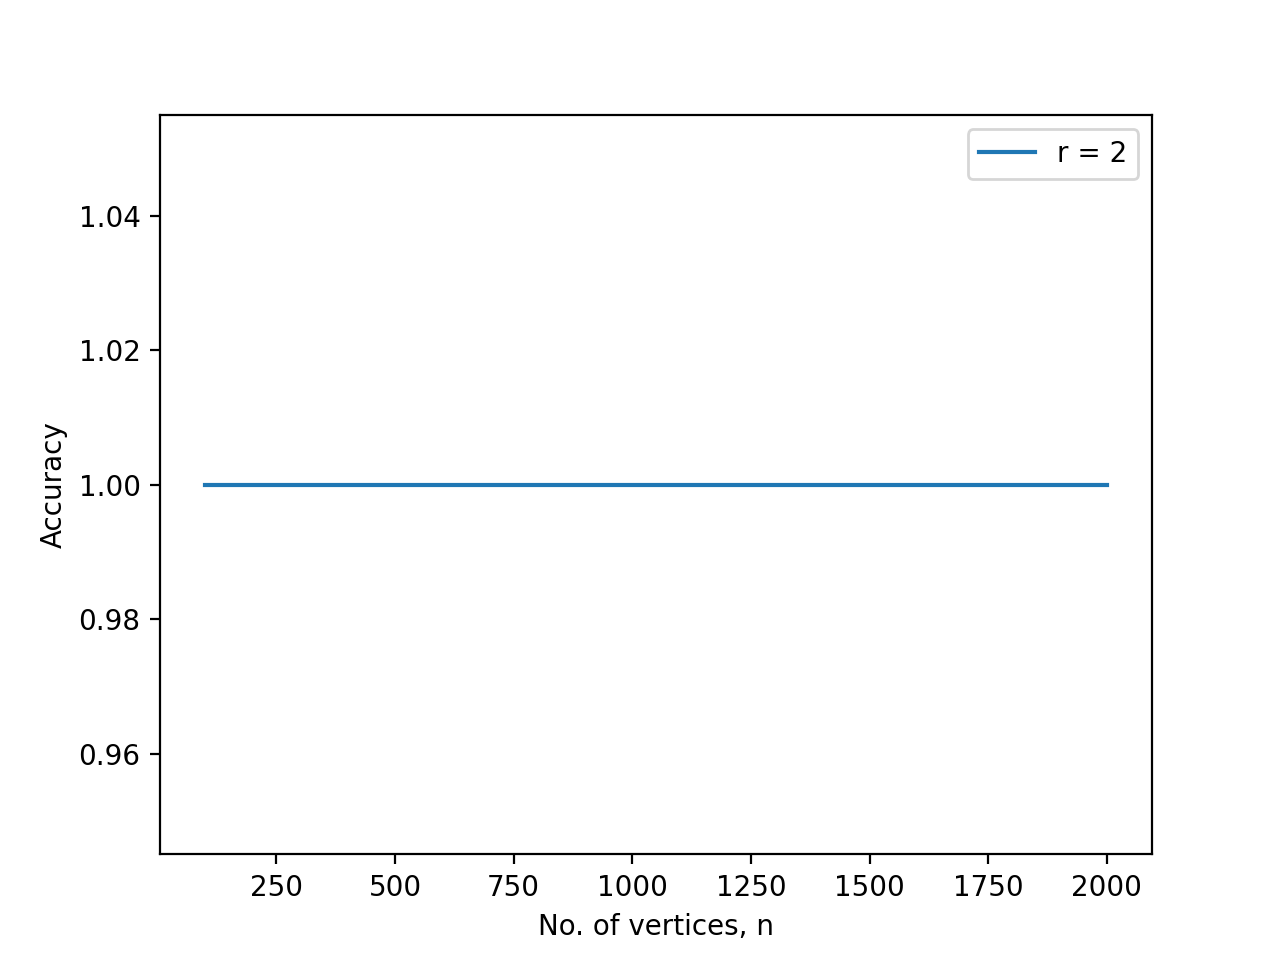
\includegraphics[width=0.9\linewidth, height=7cm]{pic/ch-Dham/accr.png}
\caption{No. of Attemps plot}
\label{fig:dham:accr}
\end{subfigure}

\caption{DHAM running on instances from the $D_{n, m}$ model}
\label{fig:dham:plots}
\end{figure}


We now try to increase the number of edges in the input graph (by varying the value of $c$). From \autoref{fig:dham:plots} we can see that the runtime does not seem to vary much, w.r.t the number of edges in the graph. This is what we would have predicted, since the algorithm considers only the first $m^*$ edges to find the cycle, so extra edges should not affect the runtime. 

\begin{figure}[H]

\centering
\includegraphics[width=0.9\linewidth, height=8cm]{pic/ch-Dham/varyc.png}
\caption{Varying the value of c}
\label{fig:dham:varyc}

\end{figure}

Another interesting thing to study is to modify the algorithm to consider more than just the first $m^*$ edges. If we increase the number of edges by a constant factor, we could potentially see some constant factor improvements in runtime, since having access to a bigger set of edges could make a lot of our procedures terminate successfully sooner. 

Running the test (\autoref{fig:dham:varya_time}) shows us that there is no such improvement in the runtime. But, what we see in \autoref{fig:dham:varya_atmp} is that the average number of times we need to run the algorithm to find a cycle drops significantly, down to almost 1, just by considering the first $2m^*$ edges instead of just the first $m^*$. 


\begin{figure}[ht]

\begin{subfigure}{\textwidth}
\centering
\includegraphics[width=0.9\linewidth, height=7cm]{pic/ch-Dham/varya_time.png}
\caption{Modifying DHAM to consider more edges - runtime}
\label{fig:dham:varya_time}
\end{subfigure}
\begin{subfigure}{\textwidth}
\centering
\includegraphics[width=0.9\linewidth, height=7cm]{pic/ch-Dham/varya_atmp.png}
\caption{Modifying DHAM to consider more edges - avg no.of attempts}
\label{fig:dham:varya_atmp}
\end{subfigure}

\caption{modified DHAM}
\label{fig:dham:expt}
\end{figure}